\documentclass{standalone}
\usepackage{tikz}
\usetikzlibrary{patterns, positioning}


\begin{document}
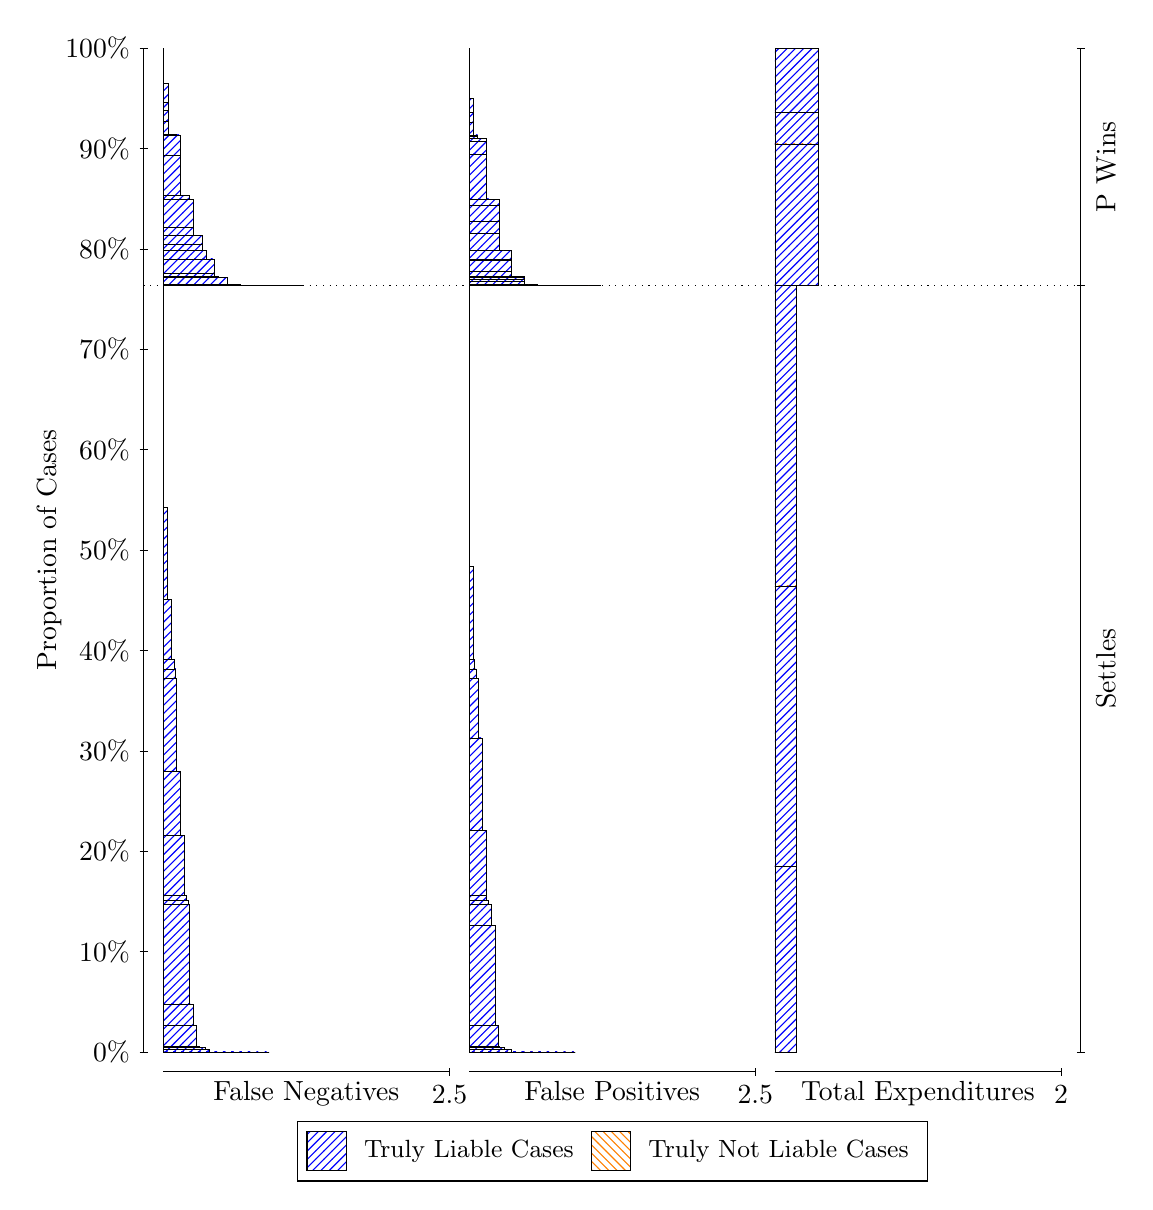
\begin{tikzpicture}
\draw[black, very thin] (1.5,1.75) -- (1.5,14.5);
\node[rotate=90, text=black, anchor=center] at (0.3, 8.125) {Proportion of Cases};
\draw[black, very thin] (1.45,1.75) -- (1.55,1.75);
\node[text=black, anchor=east] at (1.45, 1.75) {0\%};
\draw[black, very thin] (1.45,3.025) -- (1.55,3.025);
\node[text=black, anchor=east] at (1.45, 3.025) {10\%};
\draw[black, very thin] (1.45,4.3) -- (1.55,4.3);
\node[text=black, anchor=east] at (1.45, 4.3) {20\%};
\draw[black, very thin] (1.45,5.575) -- (1.55,5.575);
\node[text=black, anchor=east] at (1.45, 5.575) {30\%};
\draw[black, very thin] (1.45,6.85) -- (1.55,6.85);
\node[text=black, anchor=east] at (1.45, 6.85) {40\%};
\draw[black, very thin] (1.45,8.125) -- (1.55,8.125);
\node[text=black, anchor=east] at (1.45, 8.125) {50\%};
\draw[black, very thin] (1.45,9.4) -- (1.55,9.4);
\node[text=black, anchor=east] at (1.45, 9.4) {60\%};
\draw[black, very thin] (1.45,10.675) -- (1.55,10.675);
\node[text=black, anchor=east] at (1.45, 10.675) {70\%};
\draw[black, very thin] (1.45,11.95) -- (1.55,11.95);
\node[text=black, anchor=east] at (1.45, 11.95) {80\%};
\draw[black, very thin] (1.45,13.225) -- (1.55,13.225);
\node[text=black, anchor=east] at (1.45, 13.225) {90\%};
\draw[black, very thin] (1.45,14.5) -- (1.55,14.5);
\node[text=black, anchor=east] at (1.45, 14.5) {100\%};

\draw[black, very thin] (13.4,1.75) -- (13.4,14.5);
\draw[black, very thin] (13.35,1.75) -- (13.45,1.75);
\node[anchor=west] at (13.35, 1.75) {};
\draw[black, very thin] (13.35,11.482) -- (13.45,11.482);
\node[anchor=west] at (13.35, 11.482) {};
\draw[black, very thin] (13.35,14.5) -- (13.45,14.5);
\node[anchor=west] at (13.35, 14.5) {};

\draw[black, very thin, pattern color=blue, pattern=north east lines] (1.75,1.75) rectangle (3.0943,1.75);
\draw[black, very thin, pattern color=blue, pattern=north east lines] (1.75,1.75) rectangle (2.9329,1.75);
\draw[black, very thin, pattern color=blue, pattern=north east lines] (1.75,1.75) rectangle (2.8763,1.75);
\draw[black, very thin, pattern color=blue, pattern=north east lines] (1.75,1.75) rectangle (2.7714,1.75);
\draw[black, very thin, pattern color=blue, pattern=north east lines] (1.75,1.75) rectangle (2.7149,1.75);
\draw[black, very thin, pattern color=blue, pattern=north east lines] (1.75,1.75) rectangle (2.6583,1.75);
\draw[black, very thin, pattern color=blue, pattern=north east lines] (1.75,1.75) rectangle (2.6099,1.75);
\draw[black, very thin, pattern color=blue, pattern=north east lines] (1.75,1.75) rectangle (2.5857,1.75);
\draw[black, very thin, pattern color=blue, pattern=north east lines] (1.75,1.75) rectangle (2.5534,1.75);
\draw[black, very thin, pattern color=blue, pattern=north east lines] (1.75,1.75) rectangle (2.4969,1.7506);
\draw[black, very thin, pattern color=blue, pattern=north east lines] (1.75,1.7506) rectangle (2.4484,1.7511);
\draw[black, very thin, pattern color=blue, pattern=north east lines] (1.75,1.7511) rectangle (2.4242,1.7511);
\draw[black, very thin, pattern color=blue, pattern=north east lines] (1.75,1.7511) rectangle (2.3919,1.7513);
\draw[black, very thin, pattern color=blue, pattern=north east lines] (1.75,1.7513) rectangle (2.3677,1.7518);
\draw[black, very thin, pattern color=blue, pattern=north east lines] (1.75,1.7518) rectangle (2.3354,1.7784);
\draw[black, very thin, pattern color=blue, pattern=north east lines] (1.75,1.7784) rectangle (2.2869,1.8046);
\draw[black, very thin, pattern color=blue, pattern=north east lines] (1.75,1.8046) rectangle (2.2627,1.8046);
\draw[black, very thin, pattern color=blue, pattern=north east lines] (1.75,1.8046) rectangle (2.2304,1.8115);
\draw[black, very thin, pattern color=blue, pattern=north east lines] (1.75,1.8115) rectangle (2.2062,1.8194);
\draw[black, very thin, pattern color=blue, pattern=north east lines] (1.75,1.8194) rectangle (2.1739,2.0889);
\draw[black, very thin, pattern color=blue, pattern=north east lines] (1.75,2.0889) rectangle (2.1254,2.3607);
\draw[black, very thin, pattern color=blue, pattern=north east lines] (1.75,2.3607) rectangle (2.1012,2.3608);
\draw[black, very thin, pattern color=blue, pattern=north east lines] (1.75,2.3608) rectangle (2.077,3.6239);
\draw[black, very thin, pattern color=blue, pattern=north east lines] (1.75,3.6239) rectangle (2.0689,3.6823);
\draw[black, very thin, pattern color=blue, pattern=north east lines] (1.75,3.6823) rectangle (2.0447,3.7414);
\draw[black, very thin, pattern color=blue, pattern=north east lines] (1.75,3.7414) rectangle (2.0124,4.4983);
\draw[black, very thin, pattern color=blue, pattern=north east lines] (1.75,4.4983) rectangle (1.964,5.3184);
\draw[black, very thin, pattern color=blue, pattern=north east lines] (1.75,5.3184) rectangle (1.9397,5.3189);
\draw[black, very thin, pattern color=blue, pattern=north east lines] (1.75,5.3189) rectangle (1.9155,6.4948);
\draw[black, very thin, pattern color=blue, pattern=north east lines] (1.75,6.4948) rectangle (1.9074,6.6161);
\draw[black, very thin, pattern color=blue, pattern=north east lines] (1.75,6.6161) rectangle (1.8832,6.7373);
\draw[black, very thin, pattern color=blue, pattern=north east lines] (1.75,6.7373) rectangle (1.8509,7.4943);
\draw[black, very thin, pattern color=blue, pattern=north east lines] (1.75,7.4943) rectangle (1.8025,8.6701);
\draw[black, very thin, pattern color=blue, pattern=north east lines] (1.75,8.6701) rectangle (1.7783,8.6706);
\draw[black, very thin, pattern color=blue, pattern=north east lines] (1.75,8.6706) rectangle (1.754,9.4907);
\draw[black, very thin, pattern color=orange, pattern=north west lines] (1.75,9.4907) rectangle (1.75,9.4907);
\draw[black, very thin, pattern color=blue, pattern=north east lines] (1.75,9.4907) rectangle (1.75,11.482);
\draw[black, very thin, pattern color=blue, pattern=north east lines] (1.75,11.482) rectangle (3.5303,11.482);
\draw[black, very thin, pattern color=blue, pattern=north east lines] (1.75,11.482) rectangle (3.3689,11.482);
\draw[black, very thin, pattern color=blue, pattern=north east lines] (1.75,11.482) rectangle (3.2074,11.482);
\draw[black, very thin, pattern color=blue, pattern=north east lines] (1.75,11.482) rectangle (3.0984,11.482);
\draw[black, very thin, pattern color=blue, pattern=north east lines] (1.75,11.482) rectangle (3.0459,11.482);
\draw[black, very thin, pattern color=blue, pattern=north east lines] (1.75,11.482) rectangle (2.9369,11.482);
\draw[black, very thin, pattern color=blue, pattern=north east lines] (1.75,11.482) rectangle (2.8844,11.483);
\draw[black, very thin, pattern color=blue, pattern=north east lines] (1.75,11.483) rectangle (2.8844,11.484);
\draw[black, very thin, pattern color=blue, pattern=north east lines] (1.75,11.484) rectangle (2.7754,11.484);
\draw[black, very thin, pattern color=blue, pattern=north east lines] (1.75,11.484) rectangle (2.7754,11.484);
\draw[black, very thin, pattern color=blue, pattern=north east lines] (1.75,11.484) rectangle (2.7229,11.491);
\draw[black, very thin, pattern color=blue, pattern=north east lines] (1.75,11.491) rectangle (2.7229,11.501);
\draw[black, very thin, pattern color=blue, pattern=north east lines] (1.75,11.501) rectangle (2.6139,11.501);
\draw[black, very thin, pattern color=blue, pattern=north east lines] (1.75,11.501) rectangle (2.5614,11.591);
\draw[black, very thin, pattern color=blue, pattern=north east lines] (1.75,11.591) rectangle (2.4524,11.595);
\draw[black, very thin, pattern color=blue, pattern=north east lines] (1.75,11.595) rectangle (2.4524,11.6);
\draw[black, very thin, pattern color=blue, pattern=north east lines] (1.75,11.6) rectangle (2.4,11.638);
\draw[black, very thin, pattern color=blue, pattern=north east lines] (1.75,11.638) rectangle (2.4,11.823);
\draw[black, very thin, pattern color=blue, pattern=north east lines] (1.75,11.823) rectangle (2.291,11.931);
\draw[black, very thin, pattern color=blue, pattern=north east lines] (1.75,11.931) rectangle (2.2385,12.003);
\draw[black, very thin, pattern color=blue, pattern=north east lines] (1.75,12.003) rectangle (2.2385,12.12);
\draw[black, very thin, pattern color=blue, pattern=north east lines] (1.75,12.12) rectangle (2.1295,12.224);
\draw[black, very thin, pattern color=blue, pattern=north east lines] (1.75,12.224) rectangle (2.1295,12.584);
\draw[black, very thin, pattern color=blue, pattern=north east lines] (1.75,12.584) rectangle (2.077,12.633);
\draw[black, very thin, pattern color=blue, pattern=north east lines] (1.75,12.633) rectangle (1.968,13.136);
\draw[black, very thin, pattern color=blue, pattern=north east lines] (1.75,13.136) rectangle (1.968,13.398);
\draw[black, very thin, pattern color=blue, pattern=north east lines] (1.75,13.398) rectangle (1.9155,13.402);
\draw[black, very thin, pattern color=blue, pattern=north east lines] (1.75,13.402) rectangle (1.8065,13.574);
\draw[black, very thin, pattern color=blue, pattern=north east lines] (1.75,13.574) rectangle (1.8065,13.704);
\draw[black, very thin, pattern color=blue, pattern=north east lines] (1.75,13.704) rectangle (1.8065,13.808);
\draw[black, very thin, pattern color=blue, pattern=north east lines] (1.75,13.808) rectangle (1.8065,14.051);
\draw[black, very thin, pattern color=blue, pattern=north east lines] (1.75,14.051) rectangle (1.754,14.051);
\draw[black, very thin, pattern color=orange, pattern=north west lines] (1.75,14.051) rectangle (1.75,14.051);
\draw[black, very thin, pattern color=blue, pattern=north east lines] (1.75,14.051) rectangle (1.75,14.5);
\draw[black, very thin, pattern color=orange, pattern=north west lines] (5.6333,1.75) rectangle (6.9777,1.75);
\draw[black, very thin, pattern color=blue, pattern=north east lines] (5.6333,1.75) rectangle (6.9777,1.75);
\draw[black, very thin, pattern color=blue, pattern=north east lines] (5.6333,1.75) rectangle (6.8162,1.75);
\draw[black, very thin, pattern color=orange, pattern=north west lines] (5.6333,1.75) rectangle (6.687,1.75);
\draw[black, very thin, pattern color=blue, pattern=north east lines] (5.6333,1.75) rectangle (6.687,1.75);
\draw[black, very thin, pattern color=blue, pattern=north east lines] (5.6333,1.75) rectangle (6.6547,1.75);
\draw[black, very thin, pattern color=blue, pattern=north east lines] (5.6333,1.75) rectangle (6.5255,1.75);
\draw[black, very thin, pattern color=blue, pattern=north east lines] (5.6333,1.75) rectangle (6.4932,1.75);
\draw[black, very thin, pattern color=orange, pattern=north west lines] (5.6333,1.75) rectangle (6.469,1.75);
\draw[black, very thin, pattern color=blue, pattern=north east lines] (5.6333,1.75) rectangle (6.469,1.75);
\draw[black, very thin, pattern color=orange, pattern=north west lines] (5.6333,1.75) rectangle (6.3963,1.75);
\draw[black, very thin, pattern color=blue, pattern=north east lines] (5.6333,1.75) rectangle (6.3963,1.75);
\draw[black, very thin, pattern color=blue, pattern=north east lines] (5.6333,1.75) rectangle (6.364,1.75);
\draw[black, very thin, pattern color=blue, pattern=north east lines] (5.6333,1.75) rectangle (6.3317,1.7505);
\draw[black, very thin, pattern color=blue, pattern=north east lines] (5.6333,1.7505) rectangle (6.3075,1.7505);
\draw[black, very thin, pattern color=blue, pattern=north east lines] (5.6333,1.7505) rectangle (6.2349,1.7511);
\draw[black, very thin, pattern color=blue, pattern=north east lines] (5.6333,1.7511) rectangle (6.2026,1.7513);
\draw[black, very thin, pattern color=orange, pattern=north west lines] (5.6333,1.7513) rectangle (6.1783,1.7513);
\draw[black, very thin, pattern color=blue, pattern=north east lines] (5.6333,1.7513) rectangle (6.1783,1.7518);
\draw[black, very thin, pattern color=blue, pattern=north east lines] (5.6333,1.7518) rectangle (6.1703,1.7781);
\draw[black, very thin, pattern color=blue, pattern=north east lines] (5.6333,1.7781) rectangle (6.146,1.7781);
\draw[black, very thin, pattern color=blue, pattern=north east lines] (5.6333,1.7781) rectangle (6.0734,1.8046);
\draw[black, very thin, pattern color=blue, pattern=north east lines] (5.6333,1.8046) rectangle (6.0411,1.8115);
\draw[black, very thin, pattern color=blue, pattern=north east lines] (5.6333,1.8115) rectangle (6.0169,1.8194);
\draw[black, very thin, pattern color=blue, pattern=north east lines] (5.6333,1.8194) rectangle (6.0088,2.0912);
\draw[black, very thin, pattern color=blue, pattern=north east lines] (5.6333,2.0912) rectangle (5.9846,2.0913);
\draw[black, very thin, pattern color=orange, pattern=north west lines] (5.6333,2.0913) rectangle (5.9603,2.0913);
\draw[black, very thin, pattern color=blue, pattern=north east lines] (5.6333,2.0913) rectangle (5.9603,3.3544);
\draw[black, very thin, pattern color=blue, pattern=north east lines] (5.6333,3.3544) rectangle (5.9119,3.6239);
\draw[black, very thin, pattern color=blue, pattern=north east lines] (5.6333,3.6239) rectangle (5.8796,3.6823);
\draw[black, very thin, pattern color=blue, pattern=north east lines] (5.6333,3.6823) rectangle (5.8554,3.7414);
\draw[black, very thin, pattern color=blue, pattern=north east lines] (5.6333,3.7414) rectangle (5.8473,4.5614);
\draw[black, very thin, pattern color=blue, pattern=north east lines] (5.6333,4.5614) rectangle (5.8231,4.562);
\draw[black, very thin, pattern color=blue, pattern=north east lines] (5.6333,4.562) rectangle (5.7989,5.7378);
\draw[black, very thin, pattern color=blue, pattern=north east lines] (5.6333,5.7378) rectangle (5.7504,6.4948);
\draw[black, very thin, pattern color=blue, pattern=north east lines] (5.6333,6.4948) rectangle (5.7181,6.616);
\draw[black, very thin, pattern color=blue, pattern=north east lines] (5.6333,6.616) rectangle (5.6939,6.7373);
\draw[black, very thin, pattern color=blue, pattern=north east lines] (5.6333,6.7373) rectangle (5.6858,7.9131);
\draw[black, very thin, pattern color=blue, pattern=north east lines] (5.6333,7.9131) rectangle (5.6616,7.9137);
\draw[black, very thin, pattern color=blue, pattern=north east lines] (5.6333,7.9137) rectangle (5.6374,8.7338);
\draw[black, very thin, pattern color=blue, pattern=north east lines] (5.6333,8.7338) rectangle (5.6333,11.482);
\draw[black, very thin, pattern color=orange, pattern=north west lines] (5.6333,11.482) rectangle (7.3047,11.482);
\draw[black, very thin, pattern color=blue, pattern=north east lines] (5.6333,11.482) rectangle (7.3047,11.482);
\draw[black, very thin, pattern color=orange, pattern=north west lines] (5.6333,11.482) rectangle (7.1432,11.482);
\draw[black, very thin, pattern color=blue, pattern=north east lines] (5.6333,11.482) rectangle (7.1432,11.482);
\draw[black, very thin, pattern color=orange, pattern=north west lines] (5.6333,11.482) rectangle (6.9817,11.482);
\draw[black, very thin, pattern color=blue, pattern=north east lines] (5.6333,11.482) rectangle (6.9817,11.482);
\draw[black, very thin, pattern color=blue, pattern=north east lines] (5.6333,11.482) rectangle (6.9817,11.482);
\draw[black, very thin, pattern color=blue, pattern=north east lines] (5.6333,11.482) rectangle (6.9817,11.482);
\draw[black, very thin, pattern color=orange, pattern=north west lines] (5.6333,11.482) rectangle (6.8202,11.482);
\draw[black, very thin, pattern color=blue, pattern=north east lines] (5.6333,11.482) rectangle (6.8202,11.482);
\draw[black, very thin, pattern color=blue, pattern=north east lines] (5.6333,11.482) rectangle (6.8202,11.482);
\draw[black, very thin, pattern color=orange, pattern=north west lines] (5.6333,11.482) rectangle (6.6587,11.482);
\draw[black, very thin, pattern color=blue, pattern=north east lines] (5.6333,11.482) rectangle (6.6587,11.483);
\draw[black, very thin, pattern color=blue, pattern=north east lines] (5.6333,11.483) rectangle (6.6587,11.484);
\draw[black, very thin, pattern color=blue, pattern=north east lines] (5.6333,11.484) rectangle (6.4973,11.49);
\draw[black, very thin, pattern color=orange, pattern=north west lines] (5.6333,11.49) rectangle (6.4973,11.49);
\draw[black, very thin, pattern color=blue, pattern=north east lines] (5.6333,11.49) rectangle (6.4973,11.494);
\draw[black, very thin, pattern color=blue, pattern=north east lines] (5.6333,11.494) rectangle (6.4973,11.501);
\draw[black, very thin, pattern color=orange, pattern=north west lines] (5.6333,11.501) rectangle (6.3883,11.501);
\draw[black, very thin, pattern color=blue, pattern=north east lines] (5.6333,11.501) rectangle (6.3883,11.501);
\draw[black, very thin, pattern color=blue, pattern=north east lines] (5.6333,11.501) rectangle (6.3358,11.532);
\draw[black, very thin, pattern color=blue, pattern=north east lines] (5.6333,11.532) rectangle (6.3358,11.559);
\draw[black, very thin, pattern color=orange, pattern=north west lines] (5.6333,11.559) rectangle (6.3358,11.559);
\draw[black, very thin, pattern color=blue, pattern=north east lines] (5.6333,11.559) rectangle (6.3358,11.584);
\draw[black, very thin, pattern color=blue, pattern=north east lines] (5.6333,11.584) rectangle (6.3358,11.6);
\draw[black, very thin, pattern color=orange, pattern=north west lines] (5.6333,11.6) rectangle (6.2268,11.6);
\draw[black, very thin, pattern color=blue, pattern=north east lines] (5.6333,11.6) rectangle (6.2268,11.6);
\draw[black, very thin, pattern color=blue, pattern=north east lines] (5.6333,11.6) rectangle (6.2268,11.6);
\draw[black, very thin, pattern color=blue, pattern=north east lines] (5.6333,11.6) rectangle (6.1743,11.668);
\draw[black, very thin, pattern color=orange, pattern=north west lines] (5.6333,11.668) rectangle (6.1743,11.668);
\draw[black, very thin, pattern color=blue, pattern=north east lines] (5.6333,11.668) rectangle (6.1743,11.808);
\draw[black, very thin, pattern color=blue, pattern=north east lines] (5.6333,11.808) rectangle (6.1743,11.82);
\draw[black, very thin, pattern color=blue, pattern=north east lines] (5.6333,11.82) rectangle (6.1743,11.931);
\draw[black, very thin, pattern color=orange, pattern=north west lines] (5.6333,11.931) rectangle (6.0653,11.931);
\draw[black, very thin, pattern color=blue, pattern=north east lines] (5.6333,11.931) rectangle (6.0653,11.931);
\draw[black, very thin, pattern color=blue, pattern=north east lines] (5.6333,11.931) rectangle (6.0653,11.931);
\draw[black, very thin, pattern color=blue, pattern=north east lines] (5.6333,11.931) rectangle (6.0128,12.151);
\draw[black, very thin, pattern color=blue, pattern=north east lines] (5.6333,12.151) rectangle (6.0128,12.304);
\draw[black, very thin, pattern color=blue, pattern=north east lines] (5.6333,12.304) rectangle (6.0128,12.498);
\draw[black, very thin, pattern color=blue, pattern=north east lines] (5.6333,12.498) rectangle (6.0128,12.58);
\draw[black, very thin, pattern color=orange, pattern=north west lines] (5.6333,12.58) rectangle (5.9038,12.58);
\draw[black, very thin, pattern color=blue, pattern=north east lines] (5.6333,12.58) rectangle (5.9038,12.584);
\draw[black, very thin, pattern color=blue, pattern=north east lines] (5.6333,12.584) rectangle (5.9038,12.584);
\draw[black, very thin, pattern color=blue, pattern=north east lines] (5.6333,12.584) rectangle (5.8513,13.155);
\draw[black, very thin, pattern color=blue, pattern=north east lines] (5.6333,13.155) rectangle (5.8513,13.316);
\draw[black, very thin, pattern color=blue, pattern=north east lines] (5.6333,13.316) rectangle (5.8513,13.349);
\draw[black, very thin, pattern color=blue, pattern=north east lines] (5.6333,13.349) rectangle (5.7423,13.378);
\draw[black, very thin, pattern color=orange, pattern=north west lines] (5.6333,13.378) rectangle (5.7423,13.378);
\draw[black, very thin, pattern color=blue, pattern=north east lines] (5.6333,13.378) rectangle (5.7423,13.383);
\draw[black, very thin, pattern color=blue, pattern=north east lines] (5.6333,13.383) rectangle (5.7423,13.398);
\draw[black, very thin, pattern color=blue, pattern=north east lines] (5.6333,13.398) rectangle (5.6899,13.551);
\draw[black, very thin, pattern color=blue, pattern=north east lines] (5.6333,13.551) rectangle (5.6899,13.681);
\draw[black, very thin, pattern color=blue, pattern=north east lines] (5.6333,13.681) rectangle (5.6899,13.858);
\draw[black, very thin, pattern color=blue, pattern=north east lines] (5.6333,13.858) rectangle (5.6899,13.862);
\draw[black, very thin, pattern color=blue, pattern=north east lines] (5.6333,13.862) rectangle (5.6333,14.5);
\draw[black, very thin, pattern color=orange, pattern=north west lines] (9.5167,1.75) rectangle (9.7892,1.75);
\draw[black, very thin, pattern color=blue, pattern=north east lines] (9.5167,1.75) rectangle (9.7892,4.1114);
\draw[black, very thin, pattern color=orange, pattern=north west lines] (9.5167,4.1114) rectangle (9.7892,4.1114);
\draw[black, very thin, pattern color=blue, pattern=north east lines] (9.5167,4.1114) rectangle (9.7892,7.6703);
\draw[black, very thin, pattern color=orange, pattern=north west lines] (9.5167,7.6703) rectangle (9.7892,7.6703);
\draw[black, very thin, pattern color=blue, pattern=north east lines] (9.5167,7.6703) rectangle (9.7892,11.482);
\draw[black, very thin, pattern color=orange, pattern=north west lines] (9.5167,11.482) rectangle (10.062,11.482);
\draw[black, very thin, pattern color=blue, pattern=north east lines] (9.5167,11.482) rectangle (10.062,13.282);
\draw[black, very thin, pattern color=orange, pattern=north west lines] (9.5167,13.282) rectangle (10.062,13.282);
\draw[black, very thin, pattern color=blue, pattern=north east lines] (9.5167,13.282) rectangle (10.062,13.686);
\draw[black, very thin, pattern color=orange, pattern=north west lines] (9.5167,13.686) rectangle (10.062,13.686);
\draw[black, very thin, pattern color=blue, pattern=north east lines] (9.5167,13.686) rectangle (10.062,14.5);
\draw[black, dotted] (1.5,11.482) -- (13.4,11.482);
\draw[black, very thin] (1.75,1.5) -- (5.3833,1.5);
\node[text=black, anchor=north] at (3.5667, 1.5) {False Negatives};
\draw[black, very thin] (5.3833,1.45) -- (5.3833,1.55);
\node[text=black, anchor=north] at (5.3833, 1.45) {2.5};

\draw[black, very thin] (5.6333,1.5) -- (9.2667,1.5);
\node[text=black, anchor=north] at (7.45, 1.5) {False Positives};
\draw[black, very thin] (9.2667,1.45) -- (9.2667,1.55);
\node[text=black, anchor=north] at (9.2667, 1.45) {2.5};

\draw[black, very thin] (9.5167,1.5) -- (13.15,1.5);
\node[text=black, anchor=north] at (11.333, 1.5) {Total Expenditures};
\draw[black, very thin] (13.15,1.45) -- (13.15,1.55);
\node[text=black, anchor=north] at (13.15, 1.45) {2};

\node[text=black, centered, rotate=90] at (13.72, 6.616) {Settles};
\node[text=black, centered, rotate=90] at (13.72, 12.991) {P Wins};

\draw (7.449999999999999,1.5) node[draw=none] (baseCoordinate) {};
\begin{scope}[align=center]
        \matrix[scale=0.5, draw=black, below=0.5cm of baseCoordinate, nodes={draw}, column sep=0.1cm]{
            \node[rectangle, draw, minimum width=0.5cm, minimum height=0.5cm, pattern color=blue, pattern=north east lines] {}; &
            \node[draw=none, font=\small, text=black] (B) {Truly Liable Cases}; &
            \node[rectangle, draw, minimum width=0.5cm, minimum height=0.5cm, pattern color=orange, pattern=north west lines] {}; &
            \node[draw=none, font=\small, text=black] (B) {Truly Not Liable Cases}; \\
            };
\end{scope}

\end{tikzpicture}
\end{document}